% !TeX root = cluster.tex
\documentclass[paper.tex]{subfiles}

\begin{document}
	\section{Determining the Aggregation Function $A$}
	
	At first glance, the ranking of the variables $\V$ seems entirely subjective. It's not hard to buy that this aggregation function $A$ depends on the given variables, but the manner in which each variable ``positively impacts student performance'' is very dependent on what it actually \emph{means}. Unfortunately for us, the semantics of the data depend on world knowledge tied into the description, and there's no intrinsic reason to prefer any given variables over any other.
	
	Nonetheless, we might be able to exploit internal consistencies in the data to absolve ourselves of needing to manually assign ``goodness'' values to every variable. The idea is as follows: even without knowing anything about what variables do, we might be able to group them by how co-variate they are. Then, we assign each of those groupings some sort of semantics, assume that we can use the covariance of the variables as a way to carry the broad semantic interpretation back to the uninterpreted data. Even so, we haven't quite managed to escape the fact that we're building a subjective semantics from incomplete data; instead, we have subtly replaced some subjectivity with a handful of relatively palatable assumptions: 
	\begin{enumerate}[itemsep=-0.5em]
		\item The co-variance of two variables is meaningful because we humans have subconsciously picked variables that over-represent the things that we know.
		\item The distance metric is nicely behaved -- i.e., two semantically equivalent variables align well in our data, and two disparate variables have good separation.
		\item As a result, we can follow the ``centers'' of these groups nicely back into the data to find the centers of semantic categories we care about.
		\item Student success is a quantity which widely influences many of these variables.
	\end{enumerate} 
	If you're wondering why you should buy those assumptions -- it's not because they're defensible, but because they are succinct and there aren't very many of them -- very much unlike the case in which we manually assign each of the variables a weight. The point is that we don't really know what we're doing, and hope is that if we give a computer a little nudge in the right direction, it will find better weights than we ourselves could come up with. This turns out to be a common objective -- there is an entire sub-discipline of Machine Learning focused on leaning functions without any labeled examples (unsupervised) or with very few examples (weakly supervised). In both cases, the aim is to exploit internal consistencies in data. Clustering algorithms are one such family of methods.
	
	\subsection{Clustering}
	Normally, a clustering algorithm is given a list of samples, each of which has some number of features, and sorts clusters of data points -- but we want to get clusters of relevant \textit{variables}, not schools. According to standard ML practice, selecting exemplary features is usually an extremely early stage in a pipeline, and involve filtering out features based on univariate statistics\cite{univariate}. While this approach is great for prematurely eliminating rare features and reducing the dimensionality of the search space, it doesn't give us any way to estimate the true centers of the semantic clusters. As a result, we turn to some more creative applications of clustering algorithms.
	
	\subsubsection{Feature Agglomeration} The first one we consider is a hierarchical clustering algorithm that recursively merges the most similar features until the space has been reduced to the given number of dimensions. Feature agglomeration also has the additional benefit of allowing a user to specify an underlying hierarchical topology for the features, which we can get from the \texttt{data\_dictionary.yaml} file that accompanies the scorecard data set. To give readers who haven't seen the data a feel for how this tree is generated, consider the following short selection of tags from the feature dictionary:
	\begin{Verbatim}[xleftmargin=.5in]
		school.minority_serving.hispanic
		school.women_only
		admissions.admission_rate.overall
		admissions.admission_rate.by_ope_id
	\end{Verbatim}
	Each of these tags is associated to name of the column and a plain English description, and so these tags impose a natural tree structure on the feature space, which we pass to \texttt{skit-learn}'s Feature Agglomeration function.
	
	\subsubsection{K-Means Clustering}
	Usually the baseline approach for clustering problems, K-means clustering is a simple and very generally applicable algorithm. We include it here for completeness, and because it actually generates cluster centers, unlike the feature agglomeration approach, which deals with features categorically -- and for good reason. Applying K-Means is a little more complicated than one might hope because of the issue described above; a na\"{i}ve application of k-means would yield school clusters. Let's call the matrix of raw data $\mathbf{Y}$, where each row contains the statistics for a single school in a given year. The intuitive first step is to transpose the matrix, so that the old features are now samples, and vice versa. But now our averaging operations don't make any sense; we're adding together quantities with different units, some of which are categorical, others of which are continuous. The solution is to remove features without any variance, and re-scale the remaining ones such that they all have the same mean $\mu = 0$ and variance $\sigma^2 = 1$. If $I$ is our imputation method, $V$ is the variance filter, and $S$ transforms each column to unit variance, then what we're actually doing is:
	\[\texttt{k-means} \longleftarrow \Big(S \circ V \circ I (\mathbf{Y}) \Big)^T \]
	There is plenty of reason to be suspicious of this operation, but it happens to align very nicely with the feature agglomeration results, and so we interpret this agreement as a sign that it's relatively safe to use the cluster centers from the k-means method.
	
	\subsection{Clustering Results}
	Both the K-Means and Feature Agglomeration methods were run for various sizes of clusters. The feature sets that they select for each cluster size are illustrated in the figures that follow. The figure axes are generated via Principal Component Analysis (PCA\footnote{PCA is another form of unsupervized dimensionality reduction, like Feature Agglomeration, that combines features to find new axes that expose the most variance in the data}), and so the axes don't have any specific meaning -- they are just the most ingenuous axes we have for illustrating high-dimensional in two dimensions. The images are included to provide some intuition of how well the separation works, but be wary; they hide hundreds of dimensions, and intuition doesn't always generalize well.
	
	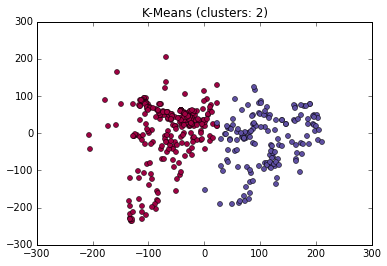
\includegraphics[width=0.5\linewidth]{images/clusters_km_2.png}
	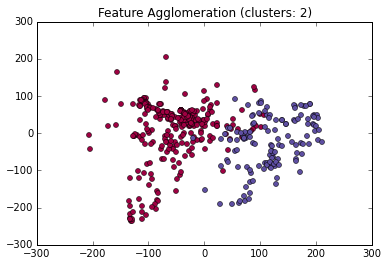
\includegraphics[width=0.5\linewidth]{images/clusters_fa_2.png}
	
	Much more telling than the visual clustering is the agreement between the two extremely different clustering algorithms. In the case of two clusters, k-means and feature agglomeration have $95.2\%$ agreement.

	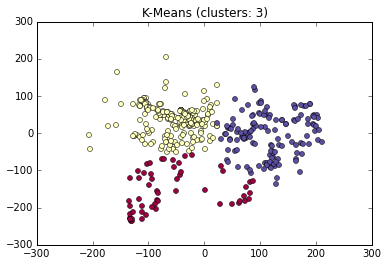
\includegraphics[width=0.5\linewidth]{images/clusters_km_3.png}
	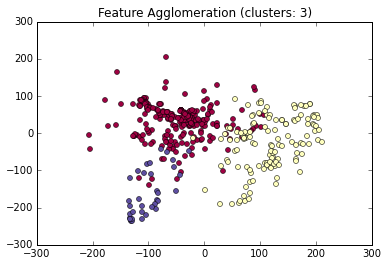
\includegraphics[width=0.5\linewidth]{images/clusters_fa_3.png}
	
	For three clusters, we still have a very good 

	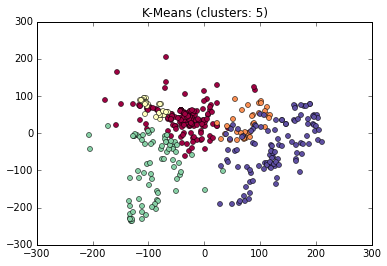
\includegraphics[width=0.5\linewidth]{images/clusters_km_5.png}
	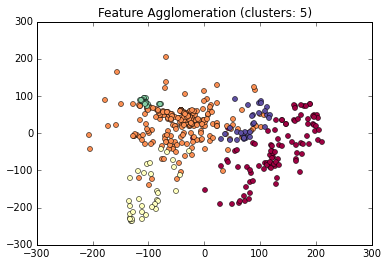
\includegraphics[width=0.5\linewidth]{images/clusters_fa_5.png}

	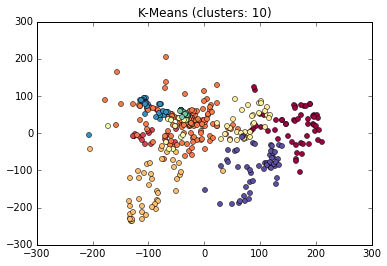
\includegraphics[width=0.5\linewidth]{images/clusters_km_10.png}
	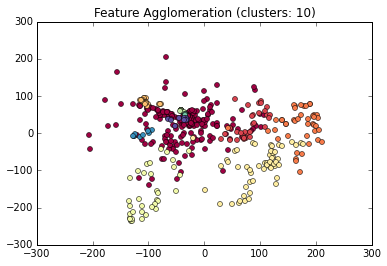
\includegraphics[width=0.5\linewidth]{images/clusters_fa_10.png}
		
	\subsection{Models to Assign Weights}
	The simplest model to consider is a linear one:
	\[A(v) = \sum_i a_i v_i \]
	
\end{document}